\documentclass{beamer}

\usepackage[utf8]{inputenc}
\usepackage[french]{babel}
\usepackage{url,graphicx,alltt}

\newcommand{\mlpost}{\textsc{Mlpost}}
\newcommand{\gmlpost}{\textsc{GMlpost}}
\newcommand{\meta}{\textsc{Metapost}}
\newcommand{\metapost}{\textsc{Metapost}}

\usetheme{Madrid}

\title{Extension de la bibliothèque Mlpost}
\author{J. Robert - G. Von Tokarski}
\date{15 mai 2009}

\begin{document}

\begin{frame}
  \maketitle

  \begin{center}
    TER Stage - Equipe 
\includegraphics[scale=0.4]{proval.png}
  \end{center}
\end{frame}

\begin{frame}{Problématique}
  Pour l'utilisateur de \LaTeX, comment réaliser des figures
  \begin{itemize}
  \item nécessitant des calculs ?
  \begin{center}
    \includegraphics[scale=0.6]{ford.mps}
  \end{center}

  \bigskip
  \item incluant des éléments \LaTeX\ arbitraires ?
    \bigskip
    \begin{center}
      \includegraphics[scale=0.8]{graph.mps}
    \end{center}
  \end{itemize}
\end{frame}

\begin{frame}[fragile]\frametitle{Metapost et MLpost}
  \meta\ est un langage (de programmation) pour construire des dessins incluant des éléments \LaTeX.

  \bigskip
  \mlpost\ est une interface Objective Caml de \meta.

  \mlpost\ est développé dans l'équipe ProVal, et est disponible en téléchargement. 
  \bigskip

  Avantages d'une interface Objective Caml par rapport à \meta:
  \begin{itemize}
  \item langage fonctionnel
  \item typage fort
  \item messages d'erreurs plus clairs
  \end{itemize}

\end{frame}

\begin{frame}[fragile]{Exemple de MLpost}  
  \begin{columns}
    \column{0.7\textwidth}\small
    \begin{verbatim}
  let simple_block =
    let b = Box.hblock ~pos:`Bot 
    [Box.tex "a"; Box.tex "A"; Box.tex "1"; 
     Box.tex "$\\pi$"] 
    in
    Box.draw b
    \end{verbatim}
    \column{0.3\textwidth}
    \includegraphics{simple_block.mps}
  \end{columns}
\end{frame}


\begin{frame}{Objectifs du TER}
  Se familiariser avec l'API.

  Ajouter/Améliorer des modules haut niveau de \mlpost.

  Documenter et tester ces modules.
  
  \vfill
  \begin{center}
    \includegraphics{architecture.mps}
  \end{center}

\end{frame}

\begin{frame}{TER Stage}
  \begin{center}
    \Huge{Nos modules}
  \end{center}
\end{frame}

\begin{frame}[fragile]{Histogramme Simple}
  \begin{columns}
    \column{0.5\linewidth}
    \begin{verbatim}
   let hist = 
     Hist.simple [3.;1.;6.]
    \end{verbatim}
    \column{0.5\linewidth}
    \begin{center}
      \includegraphics[scale=0.7]{hist1.mps}
    \end{center}
  \end{columns}
    
\end{frame}

\begin{frame}{Histogrammes comparatifs et cumulatifs}
  \begin{columns}
    \column{0.5\linewidth}
    \begin{center}
      \includegraphics% [scale=0.8]
      {hist2.mps}
    \end{center}
    
    \column{0.5\linewidth}
    \begin{center}
      \includegraphics% [scale=0.4]
      {hist3.mps}
    \end{center}
  \end{columns}
\end{frame}


\begin{frame}{API}
  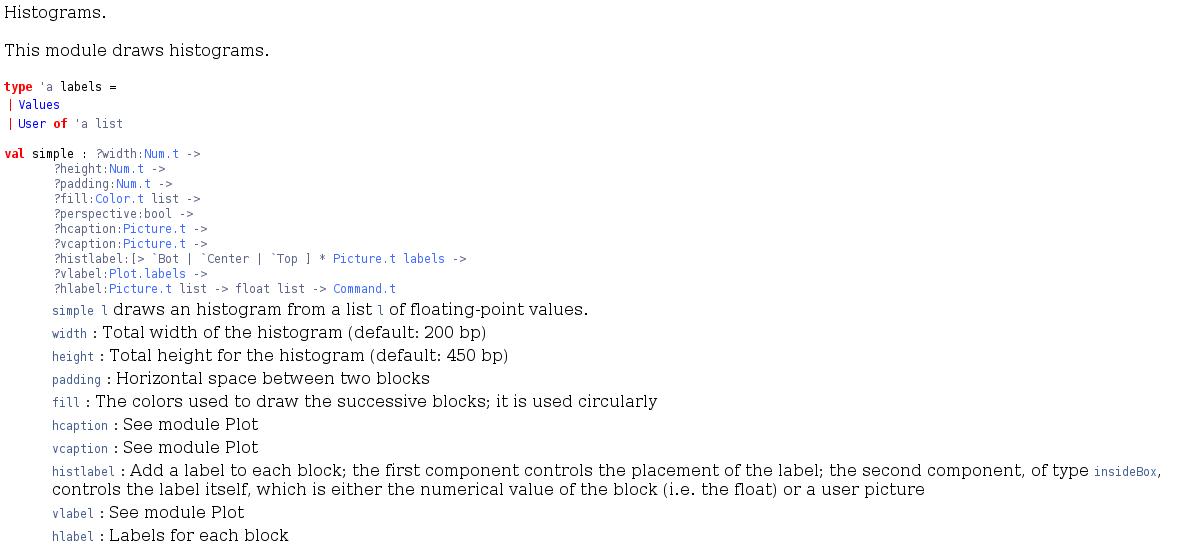
\includegraphics[scale=0.29]{ocamldoc.png}
\end{frame}

\begin{frame}[fragile]{Exemple d'utilisation}
\begin{columns}
  \column{0.5\linewidth}
  \begin{center}\footnotesize{
\begin{verbatim}
  let hist =
    let vlabel _ _ = None in
    let rot s = Picture.rotate 25. 
      (Picture.tex s) in
    Hist.stack
    ~vlabel
    ~perspective:true 
    ~padding:(bp 15.)
    ~fill:[lightred;lightblue;
      lightyellow;lightgreen]
    ~histlabel:(`Center, Hist.Values)
    ~vcaption:(Picture.tex "Dollars")
    ~hlabel:[rot "2007";rot "2008";rot "2009"]
    [[4.;5.;5.;]; [8.;3.;1.]; [2.;8.;1.;4.]]
\end{verbatim}}
      \end{center}
    
    \column{0.5\linewidth}
    \begin{center}
      \includegraphics[scale=0.7]{hist5.mps}
    \end{center}
  \end{columns}
\end{frame}
    
\begin{frame}{Structure du code}
  \begin{itemize}
  \item Code factorisé: les 3 types d'histogrammes sont principalement construits à partir de la même fonction.
  
  \bigskip
  \item Cette fonction générale prend en paramètre une liste de listes et construit un histogramme cumulatif.
  
  \bigskip
  \item Les histogrammes simples et comparatifs sont des cas particuliers.
  \end{itemize}
\end{frame}


\begin{frame}{Legend}
  \begin{columns}
    \column{0.8 \linewidth}
    \begin{center}
      \includegraphics {hist3.mps}
    \end{center}
    \column{0.2 \linewidth} \includegraphics [scale=0.8]{legend1.mps}
  \end{columns}
\end{frame}

\begin{frame}{Radar}
  \begin{center}
    \includegraphics [scale=0.6]
    {radar2.mps}
  \end{center}
\end{frame}

\begin{frame}[fragile]{Radar cumulatif}
  \begin{columns}
    \column{0.5 \linewidth}
\begin{verbatim}
  val stack :
    ?radius:Num.t ->
    ?color:Color.t list ->
    ?pen:Pen.t ->
    ?style:Dash.t list ->
    ?ticks:float ->
    ?label:string list ->
    ?scale:float list ->
    float list list -> Picture.t
\end{verbatim}
    \column{0.5 \linewidth}\includegraphics [scale=0.6]{radar1.mps}
  \end{columns}
\end{frame}


\begin{frame}[fragile]{Radar comparatif}
\begin{alltt}
  val compare :
    ?radius:Num.t ->
    ?color:Color.t list ->
    ?pen:Pen.t ->
    \color{red}?fill:bool ->
\color{black}    ?style:Dash.t list ->
    ?ticks:float ->
    ?label:string list ->
    ?scale:float list ->
    float list list -> Picture.t \color{red}list
\end{alltt}
\end{frame}


\begin{frame}[fragile]{Path}
  \begin{columns}
   % \column{0.4 \linewidth}
    
    \bigskip
    \bigskip
    \column{0.8 \linewidth}
    \begin{center}
    \includegraphics {path5.mps}
    \bigskip
    
    \includegraphics {path4.mps}
  \end{center}
    \column{0.2 \linewidth}
    \includegraphics {path1.mps}
  \end{columns}
\end{frame}


\begin{frame}[fragile]{API}
\begin{verbatim}
type orientation = 
  | Up | Down | Left | Right
  | Upn of Num.t | Downn of Num.t 
  | Leftn of Num.t | Rightn of Num.t
  
val smart_path : ?style:joint -> orientation list 
  -> Point.t -> Point.t -> t
\end{verbatim}
\end{frame}


\begin{frame}[fragile]{Path}
  \begin{columns}
    \column{0.7 \linewidth}
\begin{verbatim}
 let path = smart_path 
    ~style:jLine
    [Right;Down;Left;Down]
    (Point.pt (bp 0.,bp 0.)) 
    (Point.pt (bp 0.,bp (-30.)))
\end{verbatim}
    \column{0.3 \linewidth}
    \includegraphics [scale=1.2]
    {path2.mps}
\end{columns}
\end{frame}

\begin{frame}{Tree}
  \begin{columns}
    \column{0.5\textwidth}
    \begin{center}
      \includegraphics [scale=1.2]
      {tree2simple.mps}
    \end{center}
    \column{0.5\textwidth}
    \begin{center}
      \includegraphics [scale=1.2]
      {tree2.mps}
    \end{center}
  \end{columns}
\end{frame}

\begin{frame}[fragile]{API}
  \begin{columns}
    \column{0.7 \linewidth}
    \begin{itemize}
    \item Utilisation de l'article d'Andrew J. Kennedy: \textit{Drawing Trees}
    \item Adaptation des algorithmes pour le module
    \end{itemize}
    \column{0.3 \linewidth}
    \includegraphics[scale=1.5]{tree5.mps}

    \bigskip
    \bigskip
    \includegraphics[scale=1.2]{tree4.mps}
    \end{columns}
\end{frame}

\begin{frame}{TER Stage}
  \begin{center}
    \Huge{GMlpost}
  \end{center}
\end{frame}

\begin{frame}{GMlpost - Motivations}
  \begin{itemize}
  \item<1-> \mlpost\ permet de fabriquer des figures jolies et personnalisées.
  
  \bigskip
  
  Or il est souvent nécessaire de recompiler plusieurs fois la figure en changeant certaines valeurs pour se rapprocher du rendu souhaité. 

\bigskip

  \item<2->  \gmlpost\ est une interface graphique de \mlpost.

    \bigskip

    \gmlpost\ permet d'éditer interactivement des valeurs et des points choisis par l'utilisateur.

  \end{itemize}
\end{frame}

\begin{frame}{Screenshot}
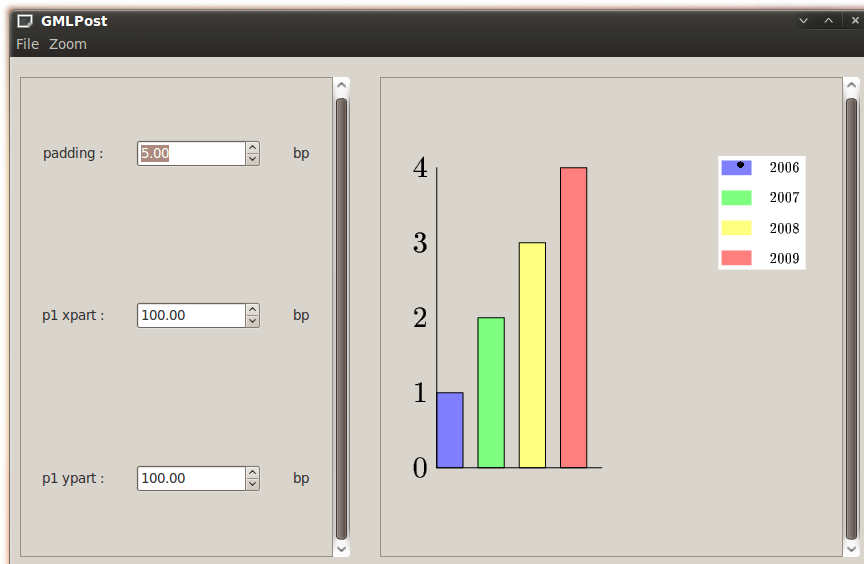
\includegraphics[scale=0.4]{screen2.png}
\end{frame}


\begin{frame}{Solution technique}
  \begin{columns}
    \column{0.5 \linewidth}
    \begin{center}
      \includegraphics [scale=0.7]{interface1.mps}
    \end{center}
    \column{0.5 \linewidth}
    \begin{center}
      \includegraphics[scale=0.7]{interface2.mps}
    \end{center}
  \end{columns}
\end{frame}

\begin{frame}{Conclusion}
  \begin{itemize}
  \item contribution significative à \mlpost
    \begin{itemize}
    \item<1-> utilisée dès à présent dans l'équipe ProVal
    \item<2-> sera distribuée avec la prochaine version de \mlpost
    \end{itemize}
    
    \bigskip
  \item<3-> sur un plan personnel
    \begin{itemize}
    \item<3-> utilisation différente d'Objective Caml (arguments optionnels, OCamldoc)
    \item<4-> découverte de lablgtk2
    \end{itemize}
  \end{itemize}
\end{frame}

\end{document}

%%% Local Variables: 
%%% mode: latex
%%% mode: whizzytex
%%% mode: flyspell
%%% ispell-local-dictionary: "francais"
%%% End: 
